% !TeX root = ../main.tex
% Add the above to each chapter to make compiling the PDF easier in some editors.
\chapter{Performance and Evaluation}\label{chapter:performance}
\section{Deployment}\label{deployment}
The proposed Android application and server have been tested on 16 devices for six days from 30.05.2019 until 04.06.2019. The version of the Android application deployed during field testing can be found on GitHub \parencite{final-version-app}. However, evaluating the \textit{lastSeen} timestamp of the users showed that only 13 installations were active after 31.05.2019. The server was deployed in the IBM Cloud as a 128 MB node.js instance. The version deployed during field testing is hosted on GitHub \parencite{final-version-server}. The latest version of the same repository provides the same functionality but includes improvements (e.g. bug-fixes, comments, ...) over the deployed version. The database was hosted as a free version at mongodb.com.

We ran 7 different aggregation requests defined in section \ref{data-aggregation-design} covering different timespans from single days to the whole time period. Also, we limited the number of participants in each aggregation to 10. The results can be found in the tables in this section and are also available in JSON format on GitHub \parencite{github-results}. The results will be discussed in Chapter \ref{results}. The results of the collection of trajectories were modified in order to protect the priacy of all research participants. We used this testing period also to improve the performance of the server as well as the Android application and to find and remove bugs. All improvements are incorporated in the most recent commits of the respective GitHub repositories.

\section{Data Consumption}
As expected, the data consumption of the Android application was low. Some research participants provided information about the app's data usage. Table \ref{data-consumption} shows the 12 collected results of this rather qualitative than quantitative analysis. Screenshots of the provided information are attached in the Appendix. On 75\% of the devices the data consumption for 6 days was below 21 MB. The highest data consumption was 376 MB and is attributable to an error that occurred on the last day of the testing period. Requests were sent multiple times during the whole period and up to unlimited times on the last day due to this error in combination with another error that was present during the whole timespan. This explains the high data consumption reported also by two other participants as the error occurred at least on three devices. The data suggests that the average data consumption in a production environment would be lower and regarding the size of our setup below 100 MB per month. Furthermore, a mobile connection is not required. In the future, the setup can be changed to use only or mostly WIFI connections.
Some few available reports about battery consumption also indicate a rather moderate battery consumption.

\begin{table}[h!]
	\centering
	\begin{tabular}{|l|l|}
		\hline
		\multicolumn{2}{|c|}{\textbf{Combined Data Consumption from 30.05.2019 - 04.06.2019}}                     \\ \hline
		\textbf{Data Consumption} & \multicolumn{1}{c|}{\textbf{Comment}}                       \\ \hline
		0 MB                               & mobile data only, WIFI unknown                              \\ \hline
		2.6 MB                             &                                                             \\ \hline
		6.19 MB                            & mobile data only, WIFI unknown                              \\ \hline
		6.29 MB                            & mobile data only, WIFI unknown                              \\ \hline
		8.18 MB                            &                                                             \\ \hline
		8.5 MB                             & From 01.04.2019 - 04.06.2019 only                           \\ \hline
		11.98 MB                           &                                                             \\ \hline
		18.53 MB                           & 16.5 MB mobile, 2.03 MB WIFI                                \\ \hline
		20.5 MB                            &                                                             \\ \hline
		75.73 MB                           & From 01.04.2019 - 04.06.2019 only, possible error candidate \\ \hline
		49.39 MB                           & mobile data only, WIFI unknown, possible error candidate    \\ \hline
		376 MB                             & Known and fixed error                                       \\ \hline
	\end{tabular}
	\caption{Overall data consumption of the Android application during the testing period.}
	\label{data-consumption}
\end{table}

\section{Aggregation Results}\label{results}
We computed the aggregation over several different timespans. We aggregated the average number of steps across all participants, the average time spent walking, running, in a vehicle or on a bicycle and collected a list of each individual's average number of steps. The results can be seen in Table \ref{results-running} - \ref{results-steps-listing}. The results from the experimental aggregation of trajectories will be discussed in Chapter \ref{trajectories}.

\subsection{Validity of results}
Excluding the value of 30.05.2019 where the collection of results started and the data of the fraction of the day before installation is not included, the average time spent walking computed in the aggregations ranges from 52 to 146 minutes per day. The average time spent walking computed for the whole timespan where data from 8 devices is included amounts to 62 minutes. At the same time, reported number of steps per day ranges from 1123 to 4682 per day, excluding outliers (see Table \ref{results-steps}). The average number of steps computed for the whole timespan with data from 5 participating devices is 3622. Taking an average speed of roughly 100 steps per minute into account \parencite{steps2}, the results from average time spent walking and average number of steps diverge by a factor of 1.7. Considering that apparently only 6 devices had a step sensor on their phone and the sample size of the steps aggregation is only about half of the sample size of the other aggregations, this deviation does not seem out of range. Furthermore there was an error computing the number of steps on at least one phone which caused some of the results to be off. Regarding Table \ref{results-steps-listing} it is clear, that the error occurred in the local aggregation process and it seems likely that only on one device this error occurred, as in each aggregation only one value is errorneous.

\begin{table}[]
	\parbox{.45\linewidth}{
		\centering
		\begin{tabular}{|l|l|l|}
			\hline
			\multicolumn{3}{|c|}{\textbf{Average number of steps per day}}          \\ \hline
			\textbf{Time period / Day} & \textbf{N} & \textbf{Value}           \\ \hline
			30.05.2019                 & 5          & 4332                     \\ \hline
			31.05.2019                 & 5          & 3440                     \\ \hline
			01.06.2019                 & 1          & 17                       \\ \hline
			03.06.2019                 & 3          & 455411                   \\ \hline
			04.06.2019                 & 3          & 1123                     \\ \hline
			30.05.2019 - 31.05.2019    & 6          & 3279                     \\ \hline
			30.05.2019 - 31.05.2019    & 5          & 4030                     \\ \hline
			30.05.2019 - 01.06.2019    & 6          & 4271                     \\ \hline
			30.05.2019 - 03.06.2019    & 5          & 643959                   \\ \hline
			30.05.2019 - 04.06.2019    & 5          & 3623                     \\ \hline
			31.05.2019 - 04.06.2019    & 3          & 4681                     \\ \hline
			01.06.2019 - 04.06.2019    & 2          & 2089                     \\ \hline
			02.04.2019 - 04.06.2019    & 3          & 326363                   \\ \hline
			03.04.2019 - 04.06.2019    & 3          & 455904                   \\ \hline
		\end{tabular}
		\caption{Average number of steps per day aggregated across all participating users for different timespans.}
		\label{results-steps}
	}
	\hfill
	\parbox{.45\linewidth}{
		\centering
		\begin{tabular}{|l|l|l|}
			\hline
			\multicolumn{3}{|c|}{\textbf{Average time spent walking {[}min{]}}}          \\ \hline
			\textbf{Time period / Day} & \textbf{N} & \textbf{Value} \\ \hline
			30.09.2019                 & 10         & 17.63                    \\ \hline
			31.05.2019                 & 10         & 97.25                    \\ \hline
			01.06.2019                 & 4          & 72.85                    \\ \hline
			03.06.2019                 & 9          & 146.49                   \\ \hline
			04.06.2019                 & 8          & 86.77                    \\ \hline
			30.05.2019 - 31.05.2019    & 10         & 63.20                    \\ \hline
			30.05.2019 - 31.05.2019    & 10         & 78.41                    \\ \hline
			30.05.2019 - 01.06.2019    & 10         & 75.14                    \\ \hline
			30.05.2019 - 03.06.2019    & 9          & 81.94                    \\ \hline
			30.05.2019 - 04.06.2019    & 8          & 61.86                    \\ \hline
			31.06.2019 - 04.06.2019    & 7          & 67.63                    \\ \hline
			01.06.2019 - 04.06.2019    & 7          & 57.44                    \\ \hline
			02.06.2019 - 04.06.2019    & 7          & 51.75                    \\ \hline
			03.06.2019 - 04.06.2019    & 7          & 64.04                    \\ \hline
		\end{tabular}
		\caption{Average time spent walking (in minutes) aggregated across all paricipating users for different timespans.}
		\label{results-walking}
	}
\end{table}

The average time spent running ranges up to only 2 minutes per day with one day having a 0 value across 8 participating devices. Most likely, only a fraction of the research participants goes running on a regular basis and probably even less take their smartphone along. This assumption reflects the low values for the average time spent running. Especially as attributing the whole average value to one device only would mean that one person conducted a run of less than 20 minutes seems unlikely, while it seems likely that quite some persons run for a short amount of time e.g. to catch a train or metro. Nevertheless, we cannot prove this assumption. It furthermore highlights, that for thorough analysis the aggregation of the mean value is not sufficient.
Similarly, the average number of steps across all participants of an aggregation is not very robust and does not provide much information. Table \ref{results-steps-listing} provides the average number of steps of each individual participating in the request. With the median ranging from 3195 to 3565 in all aggregations with more than 3 valid values and a mean number of 5205 steps in Germany \parencite{steps3} we have no doubt about the correctness of the values except the values resulting from (probably only one) errorneous device.

\begin{table}[]
	\centering
	\begin{tabular}{|l|l|l|}
		\hline
		\multicolumn{3}{|c|}{\textbf{Listing of average number of steps per day per of each participant}} \\ \hline
		\textbf{Time period / Day}         & \textbf{N}        & \textbf{Values}                          \\ \hline
		30.05.2019                         & 10                & 1661, 1246, 3195, 7714, 7842             \\ \hline
		31.05.2019                         & 10                & 2747, 775, 3924, 9203                    \\ \hline
		01.06.2019                         & 4                 & 17                                       \\ \hline
		03.06.2019                         & 9                 & 914, 1042, 1364278                       \\ \hline
		04.06.2019                         & 8                 & 1103, 13332, 934                         \\ \hline
		30.05.2019 - 31.05.2019            & 10                & 550, 2905, 3195, 775, 8828, 3419        \\ \hline
		30.05.2019 - 31.05.2019            & 10                & 550, 8828, 5145, 3195, 2433              \\ \hline
		30.05.2019 - 01.06.2019            & 10                & 8126, 3195, 283, 8828, 1629, 3565        \\ \hline
		30.05.2019 - 03.06.2019            & 9                 & 598, 3195, 1669, 8828, 3205505           \\ \hline
		30.05.2019 - 04.06.2019            & 8                 & 757, 1719, 8828, 3614, 3195              \\ \hline
		31.05.2019 - 04.06.2019            & 7                 & 757, 9203, 4084                         \\ \hline
		01.06.2019 - 04.06.2019            & 7                 & 826, 33511                               \\ \hline
		02.04.2019 - 04.06.2019            & 7                 & 974691, 1231, 3168                       \\ \hline
		03.04.2019 - 04.06.2019            & 7                 & 1364278, 1231, 2202                      \\ \hline
	\end{tabular}
	\caption{List of the average number of steps per day for each user aggregated for various timespans.}
	\label{results-steps-listing}
\end{table}

\begin{table}[]
	\parbox{.40\linewidth}{
		\centering
		\begin{tabular}{|l|l|l|}
			\hline
			\multicolumn{3}{|c|}{\textbf{Average time spent running {[}min{]}}}          \\ \hline
			\textbf{Time period / Day} & \textbf{N} & \textbf{Value} \\ \hline
			30.09.2019                 & 10         & 1.43                     \\ \hline
			31.05.2019                 & 10         & 1.21                     \\ \hline
			03.06.2019                 & 9          & 1.95                     \\ \hline
			04.06.2019                 & 8          & 0                        \\ \hline
			30.05.2019 - 31.05.2019    & 10         & 1.96                     \\ \hline
			30.05.2019 - 31.05.2019    & 10         & 1.89                     \\ \hline
			30.05.2019 - 01.06.2019    & 10         & 1.73                     \\ \hline
			30.05.2019 - 03.06.2019    & 9          & 1.79                     \\ \hline
			30.05.2019 - 04.06.2019    & 8          & 1.55                     \\ \hline
			31.06.2019 - 04.06.2019    & 7          & 0.83                     \\ \hline
			01.06.2019 - 04.06.2019    & 7          & 0.99                     \\ \hline
			02.06.2019 - 04.06.2019    & 7          & 1.05                     \\ \hline
			03.06.2019 - 04.06.2019    & 7          & 0.16                     \\ \hline
		\end{tabular}
		\caption{Average time spent running (in minutes) aggregated across all paricipating users for different timespans.}
		\label{results-running}
	}
	\hfill
	\parbox{.50\linewidth}{
		\begin{tabular}{|l|l|l|}
			\hline
			\multicolumn{3}{|c|}{\textbf{Average time spent in a vehicle {[}min{]}}}     \\ \hline
			\textbf{Time period / Day} & \textbf{N} & \textbf{Value} \\ \hline
			30.05.2019                 & 10         & 8.24                     \\ \hline
			31.05.2019                 & 10         & 119.92                   \\ \hline
			01.06.2019                 & 4          & 90.40                    \\ \hline
			03.06.2019                 & 9          & 71.74                    \\ \hline
			04.06.2019                 & 8          & 35.51                    \\ \hline
			30.05.2019 - 31.05.2019    & 10         & 68.40                    \\ \hline
			30.05.2019 - 31.05.2019    & 10         & 90.49                    \\ \hline
			30.05.2019 - 01.06.2019    & 10         & 82.19                    \\ \hline
			30.05.2019 - 03.06.2019    & 9          & 62.16                    \\ \hline
			30.05.2019 - 04.06.2019    & 8          & 59.34                    \\ \hline
			01.06.2019 - 04.06.2019    & 7          & 51.07                    \\ \hline
			31.05.2019 - 04.06.2019    & 7          & 68.20                    \\ \hline
			02.04.2019 - 04.06.2019    & 7          & 48.89                    \\ \hline
			03.04.2019 - 04.06.2019    & 7          & 45.96                    \\ \hline
		\end{tabular}
		\caption{Average time spent in a vehicle (in minutes) aggregated across all paricipating users for different timespans.}

		\label{results-vehicle}
	}
\end{table}

\begin{table}[]
	\centering
	\begin{tabular}{|l|l|l|}
		\hline
		\multicolumn{3}{|c|}{\textbf{Average time spent biking {[}min{]}}}           \\ \hline
		\textbf{Time period / Day} & \textbf{N} & \textbf{Value} \\ \hline
		30.05.2019                 & 10         & 2.29                     \\ \hline
		01.06.2019                 & 4          & 14.99                    \\ \hline
		03.06.2019                 & 9          & 31.03                    \\ \hline
		04.06.2019                 & 8          & 23.81                    \\ \hline
		30.05.2019 - 31.05.2019    & 10         & 11.10                    \\ \hline
	\end{tabular}
		\caption{Average time spent biking (in minutes) aggregated across all paricipating users for different timespans.}
	\label{results-biking}
\end{table}

The average time spent in a vehicle (including means of public transport) ranges from 36 to 120 minutes (excluding the aggregation only covering the first day). The average time spent in a vehicle computed by the aggregation covering the whole timespan is 59 minutes.
The average time spent biking ranges from 11 to 31 minutes. The aggregation across the whole timespan was errorneous and had to be discarded. Both aggregations - the time spent biking and the time spent in a vehicle seem reasonable to us, especially as all participants were active in the Munich area which is also a quite bike friendly city. Furthermore, the collected trajectories in section \ref{trajectories} show two rather long trajectories which probably contributed to the high average time spent in a vehicle in one of the aggregations.

\subsection{Implications}
The same aggregation covering the timespan from 30.05.2019 to 31.05.2019 has been computed twice for 4 of the aggregations. The results show that not only the number of participants varies but also the value varies from 4\% to 18\%. For each aggregation, the selected participants might be differnt. With a total number of 16 participants in our research, though there has to be an intersection. Nevertheless, the deviation in the same aggregation is within an acceptable range and will be more robust, when the number of participants is increased. Furthermore, the median value will be even more robust to computing the same aggregation twice. We see the same phenomena e.g. regarding the aggregations for the time spent running on 30.05.2019, 31.05.2019 and the aggregation covering both days. The aggregation covering both days yields a higher value than each single aggregation which is due to the fact of a differing underlying research population.

TODO: Compute average of steps and compare

\subsection{Inference on aggregated data}\label{inference}
Regarding the aggregations computing mean values across all participants, we do not see any possibility to infer information about the users who participated. Especially as not even the identifier of the user used by the server is published alongside with the aggregation. In addition, we showed that when repeating the same aggregation request, the user base changes and the value accordingly. Nevertheless, from the two different values for the same aggregation request, we cannot draw any inference. Also an overlapping in the aggregations e.g. 30.05.2019, 31.05.2019 and an aggregation covering both days as well as the aggregations covering the first two days and the last five days does not allow for inference in the case of mean values aggregated across all participants.
The collection of individual mean values in Table \ref{results-steps-listing} shows that with a high probability the same participant with an average value of 8828 steps per day who participated in the request covering the first two days also participated in the request covering the whole timespan. Based on the information that days with a zero value of the step counter are excluded also locally from the aggregation, we can infer that this person's phone did not register any steps after the first two days, otherwise they value in the second aggregation would have changed. Similarly, we can infer that the user with 757 steps on average per day who participated in the requests covering the whole 6 day timespan and the aggregation covering only the last 5 days probably did not register steps on the first day.
In summary, we can only infer information about the fact of some users who participated in one aggregation, did or did not participate in another aggregation. As this information is endogenous to our data-set, it can in no case be used to be linked to other data-sets in order to infer further information.
Assuming that we would also have the collected averages of all aggregations and not only steps.
Furthermore, linking different aggregations e.g. the number of steps and the time spent walking is only possible with a limited likelihood due to the following reasons. First, there is no exact match of e.g. time spent walking for a number of steps, so that always a range of values of another aggregation would fit. Next, we cannot even assure that the same user participated in both different aggregations. Assuming nevertheless that there is another data-set where the combination of walked steps, time spent walking, etc. is a quasi-identifier as defined by \parencite{k-anonymity-achieving}, the likelihood of obtaining a correct link is low due to the afore mentioned reasons and a good level of anonymity regarding k-anonymity would always be supplied naturally. And still, those aggregations do not expose raw location data / GPS data points which are usually the risk.

\subsection{Trajectories}\label{trajectories}
Using the algorithm described in Chapter \ref{local-data-aggregation} a total of 406 trajectories where computed from the raw GPS data. The experimental collection of trajectories clearly shows privacy risks as pointed out e.g. by \parencite{cellphone}, why we only publish a modified results set\footnote{Whenever the trajectory started or ended clearly in a precise private location e.g. housing or work-place, we slightly modified this trajectory. So the results do not represent actual trajectories. Nevertheless, the meaning of the results should not have changed.}. Most of the trajectories are shown in Fig. \ref{trajectories1} and \ref{trajectories2}. The complete results can also be found in the Appendix.

\begin{figure}[h!]
	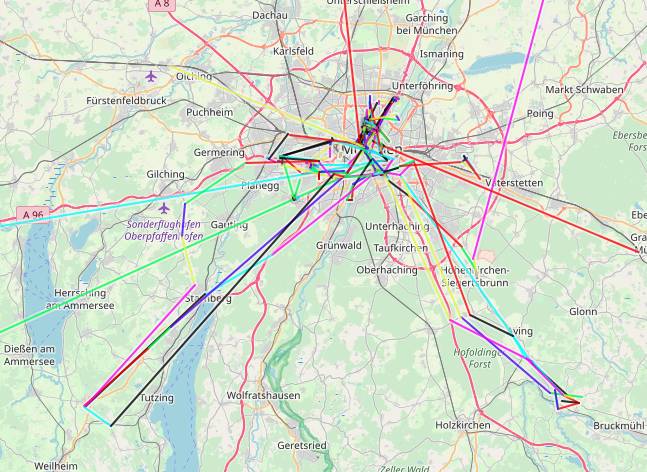
\includegraphics[width=\textwidth]{data/trajectories-2.png}
	\caption{Excerpt of all trajectories in the greater Munich area.}
	\label{trajectories1}
\end{figure}

\begin{figure}[h!]
	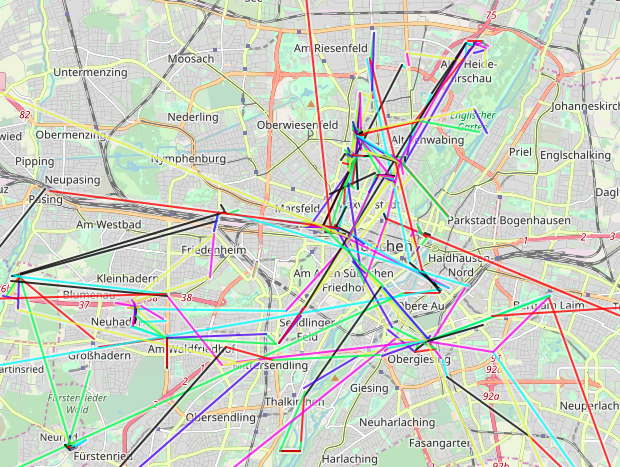
\includegraphics[width=\textwidth]{data/trajectories-3.png}
	\caption{Excerpt of all trajectories inside Munich.}
	\label{trajectories2}
\end{figure}

In more than 90\% of all cases, local trajectories obtained from one of the researchers participating devices could match an activity for more than 90\% of the time. This data data suggests that these trajectories can easily be linked locally and a change of transport system e.g. metro to bike can be identified. For example at the locations Giselastraße, Odeonsplatz and central station, many trajectories end or start. Mapping the current activity to those trajectories enables aggregations as mentioned in Chapter \ref{aggregation-schemes}. Noting that locally all data points of the trajectories are available, it is also easy to compute the distance travelled or infer a more granular transport definition e.g. train, bus, car, etc. Also, it is possible to compute how many people combine e.g. bike and car or public transport and furthermore identify, which station is most likely (in case of public transport) to be combined with bike.

The trajectories also show, that in the not anonymized data set we had at hands, often trajectories of which the endpoints did not clearly indicate an ongoing, the numeration of the trajectory indicated that they were connected. This 1. highlights the importance of list order randomization and 2. shows that our algorithm of finding trajectories still has possibilities for improvement. (TODO: Randomize order in published data set)


\section{Further scenarios e.g. Scenario Traffic Jam}
Also it would be possible to create a "travelled road" or "travelled public transport" map by aggregating the trajectories data so that there would not be multiple trajectories but each road either marked used or not used. This way it would be possible to identify that a user lives in a certain area but could not link to the work location due to obfuscation with other routes joining. This map would on the other hand allow to have a feeling of which areas are covered by the data / app. This map could also be extended with the average speed on the respective road depending on vehicle or bike and also compare whether bike is faster.

A typical scenario of google maps is o notify users about traffic jams and suggest alternate routes. The calculation of alternate routes taking traffic jams into account can clearly happen locally with the maps data. Google maps works when offline. The data about all current traffic jams can also be made publicly available through a server. Generating the data can also happen without exposing raw data: The user downloads a map containing data of the usual speeds at each street. While the user is driving, the app registers the speed and compares it in the background to the normal speed. If the speed is significantly lower, the user chooses a random list of known users and sends the signal as a request for those users to the server. They randomly according to a fixed percentage choose to inform the server about the traffic jam or forward the signal another time. The signal contains a unique id thus that the server even when receiving it muliply times knows it is from one user. If more than a threshold of signals is received, a traffic jam is "created". Also the request is not forwarded anymore after a certain time to stop it from spreading unlimited.

